% 图 58.2 —— 由 `checks/emit_hand.py` 自动拼出（probe 精测 + prims2 图元分解）
%%
% ⚠ 这是**稿子不是成品**：跑 `checks/checkhand.py 58.2` 看指标 + 看叠合图。
%%
%% ⚠ 待核：
%   · 本图 probe 报出阴影族 1 个 —— **本脚本不生成阴影**（要照原书手写）；prims2 的 strokes 里可能含阴影线，核对时留意别画重
%   · 可疑字形 9 项（空心圈 ⊙ 常被认成字母 o）—— 见文件末
%%
\documentclass[12pt]{standalone}
\usepackage{fontspec}
\setsansfont{Arial}
\newfontfamily\mfallback{DejaVu Sans}
\usepackage{tikz}
\begin{document}
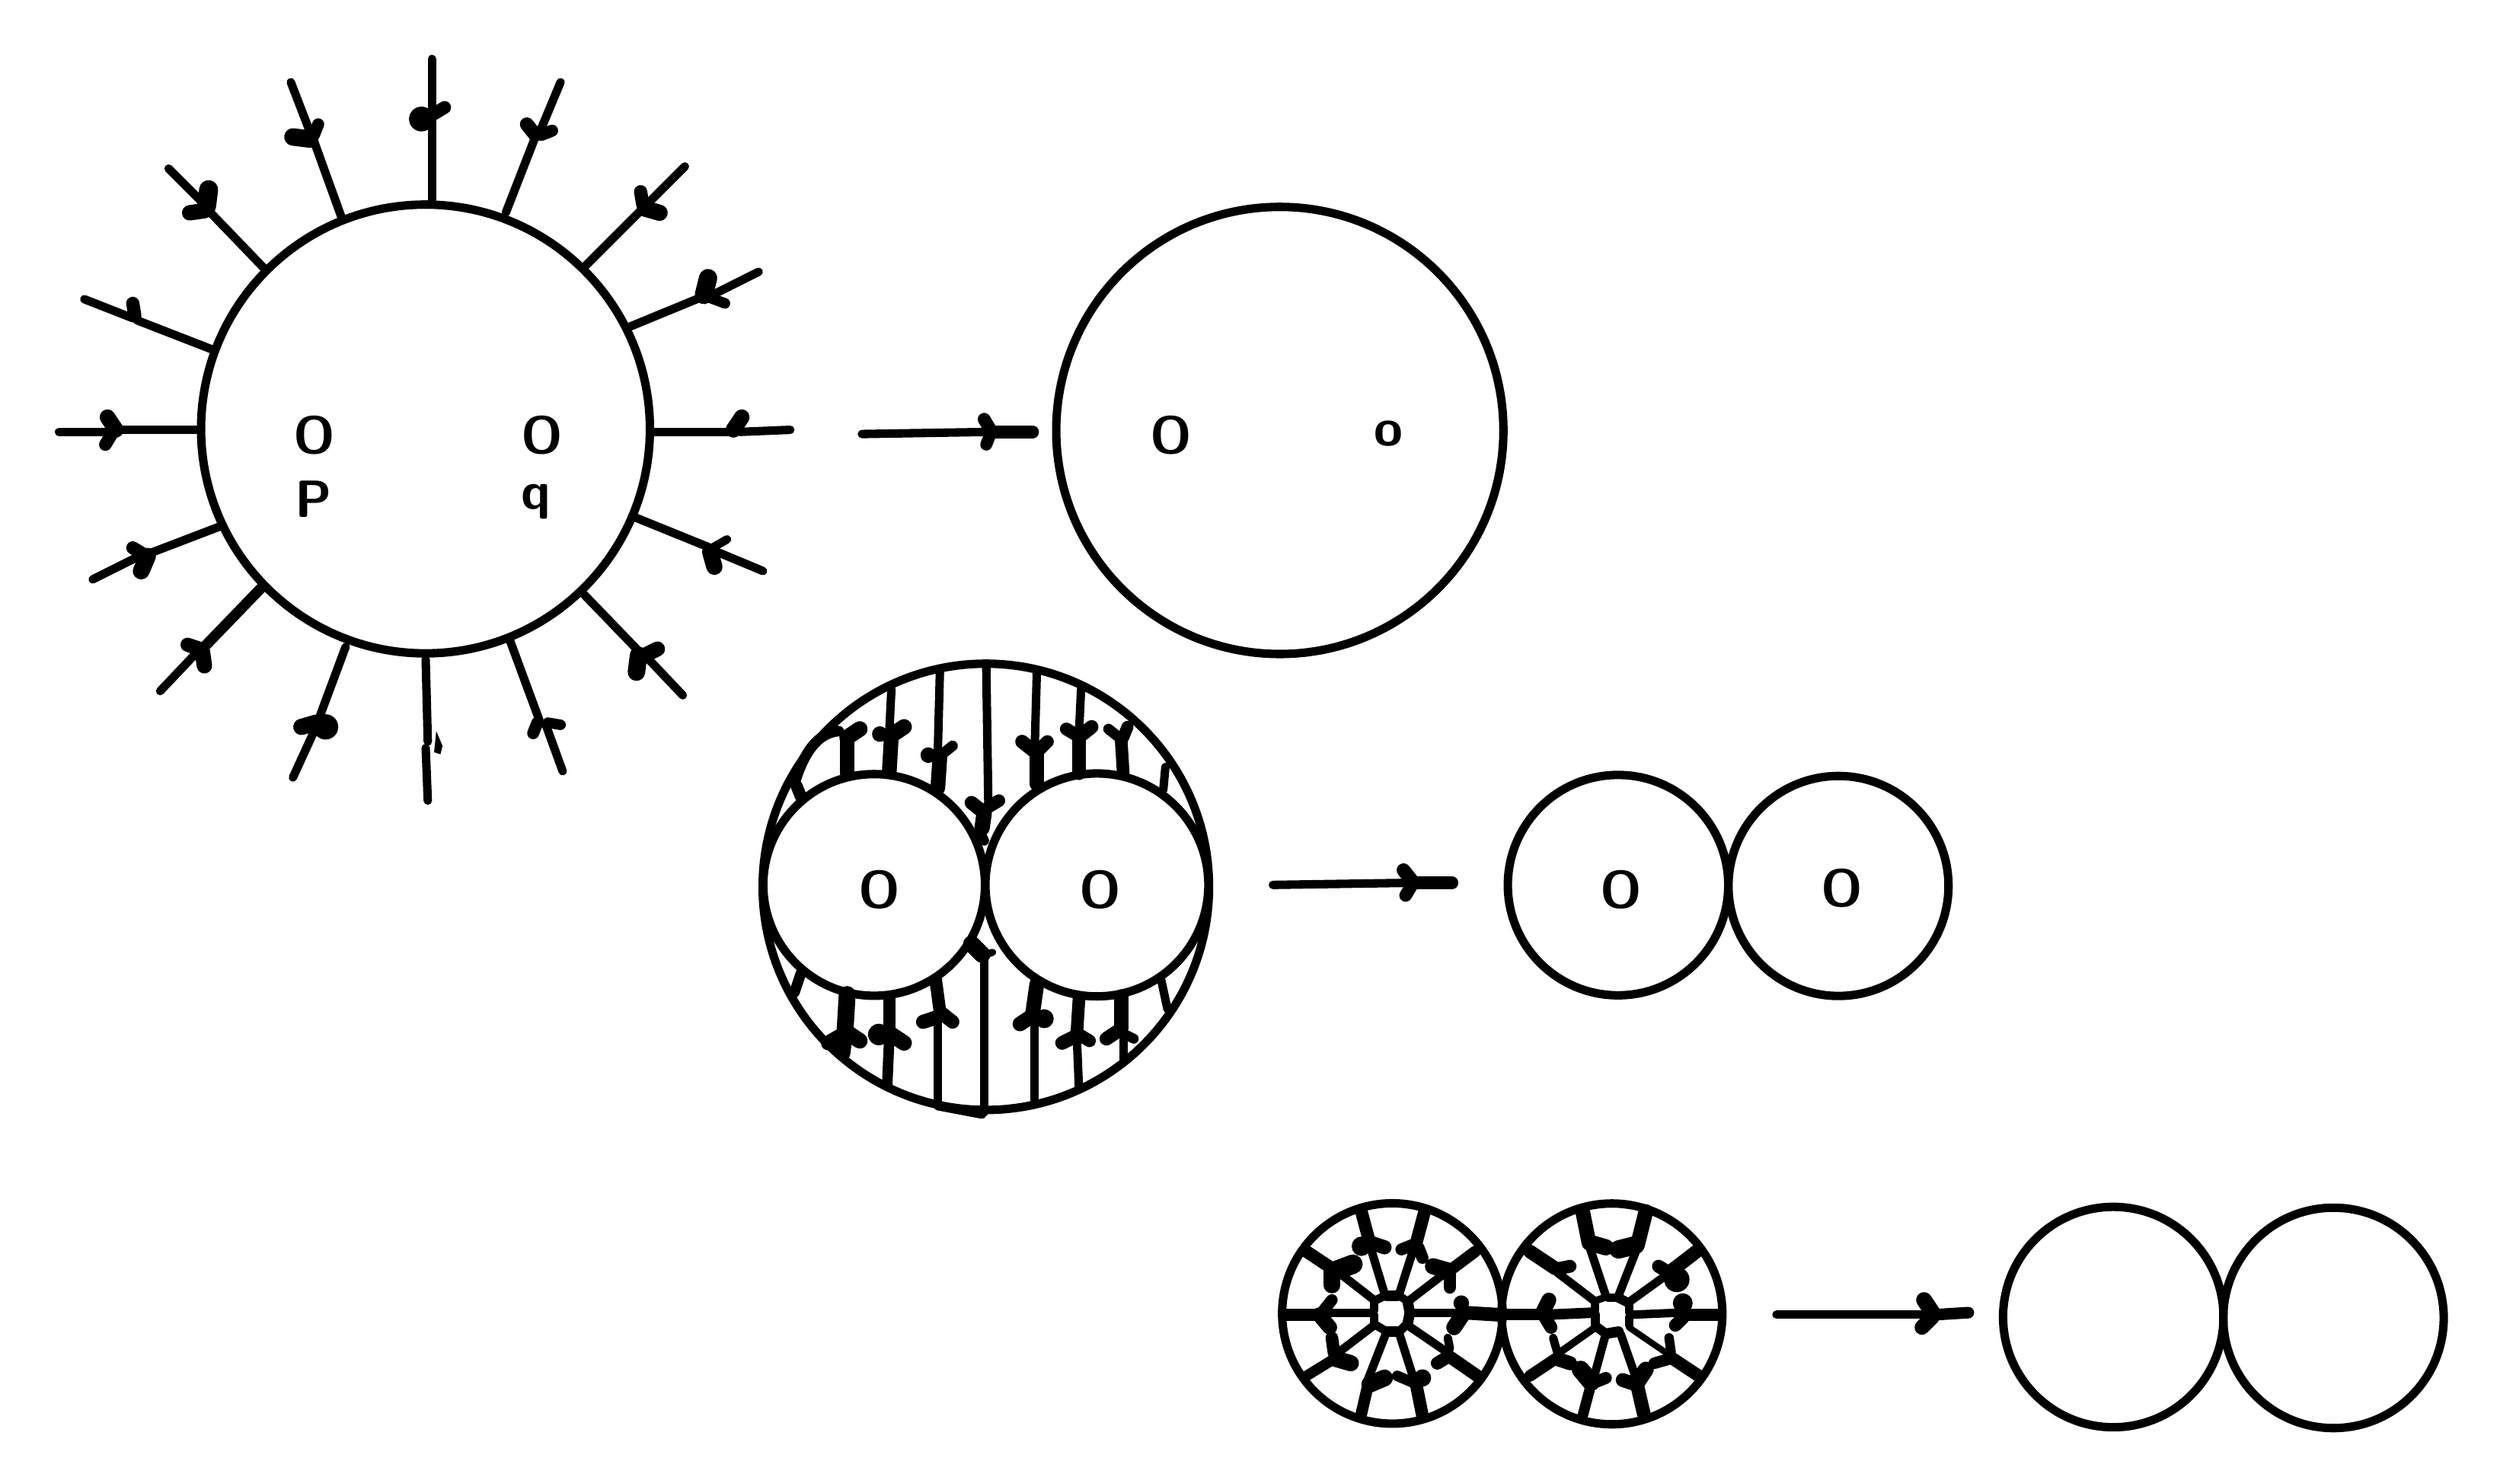
\begin{tikzpicture}[x=1pt, y=-1pt, line width=4.0pt, line cap=round, line join=round]

  %% ════ 填充区（prims2 的 fills）════
  \fill (197.0,337.0) -- (196.0,347.0) -- (199.0,348.0) -- (200.0,344.0) -- cycle;

  %% ════ 直线段（prims2 的 strokes）════
  \draw[line width=6.5pt] (770.0,661.0) -- (767.0,648.0);
  \draw[line width=5.5pt] (704.0,614.0) -- (721.0,614.0);
  \draw[line width=7.0pt] (482.0,457.0) -- (480.0,471.0);
  \draw[line width=4.0pt] (642.0,608.0) -- (642.0,612.0);
  \draw[line width=7.4pt] (419.0,485.0) -- (413.0,481.0);
  \draw[line width=4.0pt] (195.0,43.0) -- (195.0,18.0);
  \draw[line width=4.0pt] (139.0,57.0) -- (152.0,93.0);
  \draw[line width=4.0pt] (326.0,131.0) -- (350.0,119.0);
  \draw[line width=5.0pt] (326.0,131.0) -- (334.0,134.0);
  \draw[line width=4.0pt] (758.0,605.0) -- (767.0,582.0);
  \draw[line width=3.4pt] (458.0,443.0) -- (461.0,442.0);
  \draw[line width=4.0pt] (763.0,608.0) -- (781.0,595.0);
  \draw[line width=6.0pt] (464.0,370.0) -- (459.0,373.0);
  \draw[line width=4.0pt] (729.0,632.0) -- (727.0,625.0);
  \draw[line width=4.0pt] (459.0,195.0) -- (399.0,196.0);
  \draw[line width=6.5pt] (503.0,339.0) -- (508.0,335.0);
  \draw[line width=4.0pt] (85.0,194.0) -- (45.0,194.0);
  \draw[line width=6.0pt] (522.0,341.0) -- (523.0,357.0);
  \draw[line width=6.0pt] (666.0,565.0) -- (662.0,580.0);
  \draw[line width=7.0pt] (412.0,356.0) -- (413.0,339.0);
  \draw[line width=4.0pt] (729.0,594.0) -- (746.0,607.0);
  \draw[line width=4.0pt] (659.0,607.0) -- (676.0,594.0);
  \draw[line width=4.0pt] (648.0,622.0) -- (643.0,619.0);
  \draw[line width=5.0pt] (648.0,622.0) -- (653.0,622.0);
  \draw[line width=4.0pt] (648.0,622.0) -- (639.0,645.0);
  \draw[line width=4.0pt] (767.0,646.0) -- (759.0,623.0);
  \draw[line width=7.5pt] (767.0,646.0) -- (771.0,640.0);
  \draw[line width=4.0pt] (642.0,619.0) -- (625.0,632.0);
  \draw[line width=7.0pt] (480.0,472.0) -- (474.0,476.0);
  \draw[line width=6.5pt] (502.0,357.0) -- (502.0,340.0);
  \draw[line width=5.0pt] (623.0,635.0) -- (610.0,643.0);
  \draw[line width=7.0pt] (482.0,362.0) -- (482.0,347.0);
  \draw[line width=7.7pt] (296.0,89.0) -- (303.0,91.0);
  \draw[line width=4.0pt] (763.0,619.0) -- (763.0,615.0);
  \draw[line width=6.0pt] (661.0,409.0) -- (679.0,409.0);
  \draw[line width=8.3pt] (137.0,56.0) -- (129.0,55.0);
  \draw[line width=4.0pt] (249.0,334.0) -- (257.0,356.0);
  \draw[line width=7.0pt] (522.0,478.0) -- (522.0,463.0);
  \draw[line width=5.0pt] (442.0,344.0) -- (437.0,348.0);
  \draw[line width=6.7pt] (434.0,473.0) -- (428.0,475.0);
  \draw[line width=4.0pt] (412.0,337.0) -- (413.0,317.0);
  \draw[line width=5.0pt] (412.0,482.0) -- (411.0,505.0);
  \draw[line width=4.0pt] (481.0,514.0) -- (481.0,474.0);
  \draw[line width=5.0pt] (745.0,647.0) -- (741.0,662.0);
  \draw[line width=6.0pt] (806.0,614.0) -- (790.0,614.0);
  \draw[line width=7.7pt] (140.0,333.0) -- (133.0,335.0);
  \draw[line width=4.0pt] (337.0,195.0) -- (299.0,195.0);
  \draw[line width=4.0pt] (502.0,338.0) -- (503.0,317.0);
  \draw[line width=4.0pt] (833.0,614.0) -- (906.0,614.0);
  \draw[line width=4.5pt] (762.0,608.0) -- (758.0,606.0);
  \draw[line width=5.5pt] (716.0,643.0) -- (728.0,635.0);
  \draw[line width=7.7pt] (327.0,252.0) -- (329.0,259.0);
  \draw[line width=4.0pt] (230.0,91.0) -- (244.0,55.0);
  \draw[line width=6.1pt] (672.0,637.0) -- (677.0,634.0);
  \draw[line width=5.0pt] (370.0,452.0) -- (367.0,461.0);
  \draw[line width=6.1pt] (785.0,619.0) -- (789.0,615.0);
  \draw[line width=9.0pt] (89.0,80.0) -- (88.0,88.0);
  \draw[line width=5.0pt] (114.0,269.0) -- (86.0,298.0);
  \draw[line width=6.7pt] (641.0,580.0) -- (647.0,582.0);
  \draw[line width=4.0pt] (268.0,116.0) -- (295.0,89.0);
  \draw[line width=6.1pt] (483.0,346.0) -- (487.0,342.0);
  \draw[line width=5.5pt] (775.0,637.0) -- (782.0,635.0);
  \draw[line width=4.0pt] (341.0,195.0) -- (365.0,194.0);
  \draw[line width=4.0pt] (193.0,370.0) -- (192.0,345.0);
  \draw[line width=4.0pt] (752.0,605.0) -- (744.0,581.0);
  \draw[line width=4.0pt] (544.0,469.0) -- (541.0,455.0);
  \draw[line width=5.7pt] (660.0,581.0) -- (655.0,583.0);
  \draw[line width=4.0pt] (129.0,359.0) -- (140.0,335.0);
  \draw[line width=7.4pt] (684.0,614.0) -- (680.0,620.0);
  \draw[line width=8.7pt] (324.0,130.0) -- (326.0,122.0);
  \draw[line width=4.0pt] (435.0,514.0) -- (435.0,474.0);
  \draw[line width=4.0pt] (459.0,373.0) -- (458.0,306.0);
  \draw[line width=3.0pt] (782.0,633.0) -- (763.0,620.0);
  \draw[line width=7.4pt] (41.0,188.0) -- (45.0,194.0);
  \draw[line width=4.0pt] (435.0,515.0) -- (456.0,519.0);
  \draw[line width=8.0pt] (647.0,644.0) -- (640.0,647.0);
  \draw[line width=6.1pt] (726.0,620.0) -- (723.0,615.0);
  \draw[line width=4.0pt] (523.0,482.0) -- (523.0,493.0);
  \draw[line width=5.5pt] (908.0,614.0) -- (924.0,613.0);
  \draw[line width=4.0pt] (55.0,142.0) -- (91.0,156.0);
  \draw[line width=5.0pt] (658.0,618.0) -- (659.0,613.0);
  \draw[line width=8.0pt] (392.0,462.0) -- (391.0,479.0);
  \draw[line width=6.7pt] (729.0,635.0) -- (735.0,637.0);
  \draw[line width=7.0pt] (767.0,581.0) -- (771.0,565.0);
  \draw[line width=4.0pt] (481.0,345.0) -- (482.0,309.0);
  \draw[line width=4.5pt] (782.0,625.0) -- (783.0,632.0);
  \draw[line width=3.8pt] (657.0,607.0) -- (654.0,605.0);
  \draw[line width=6.0pt] (640.0,580.0) -- (636.0,565.0);
  \draw[line width=6.6pt] (760.0,645.0) -- (766.0,647.0);
  \draw[line width=6.0pt] (610.0,584.0) -- (622.0,592.0);
  \draw[line width=4.0pt] (128.0,29.0) -- (138.0,55.0);
  \draw[line width=4.0pt] (677.0,632.0) -- (658.0,619.0);
  \draw[line width=4.0pt] (682.0,613.0) -- (659.0,613.0);
  \draw[line width=6.5pt] (500.0,482.0) -- (494.0,485.0);
  \draw[line width=5.0pt] (758.0,622.0) -- (752.0,623.0);
  \draw[line width=6.1pt] (460.0,194.0) -- (457.0,189.0);
  \draw[line width=5.7pt] (523.0,340.0) -- (525.0,335.0);
  \draw[line width=5.5pt] (639.0,648.0) -- (636.0,661.0);
  \draw[line width=4.0pt] (115.0,117.0) -- (89.0,90.0);
  \draw[line width=5.7pt] (665.0,587.0) -- (663.0,582.0);
  \draw[line width=4.0pt] (746.0,645.0) -- (752.0,623.0);
  \draw[line width=4.0pt] (643.0,607.0) -- (647.0,605.0);
  \draw[line width=6.5pt] (442.0,475.0) -- (437.0,471.0);
  \draw[line width=7.3pt] (80.0,91.0) -- (87.0,90.0);
  \draw[line width=4.0pt] (289.0,145.0) -- (323.0,131.0);
  \draw[line width=7.7pt] (622.0,600.0) -- (622.0,593.0);
  \draw[line width=5.0pt] (659.0,613.0) -- (658.0,608.0);
  \draw[line width=4.0pt] (642.0,614.0) -- (642.0,618.0);
  \draw[line width=4.5pt] (747.0,619.0) -- (747.0,614.0);
  \draw[line width=6.1pt] (730.0,592.0) -- (735.0,591.0);
  \draw[line width=6.5pt] (475.0,342.0) -- (480.0,346.0);
  \draw[line width=7.3pt] (86.0,299.0) -- (87.0,306.0);
  \draw[line width=4.0pt] (328.0,250.0) -- (335.0,246.0);
  \draw[line width=7.4pt] (392.0,340.0) -- (398.0,336.0);
  \draw[line width=4.0pt] (654.0,604.0) -- (661.0,582.0);
  \draw[line width=4.0pt] (543.0,354.0) -- (542.0,365.0);
  \draw[line width=5.0pt] (516.0,336.0) -- (521.0,340.0);
  \draw[line width=4.0pt] (297.0,87.0) -- (315.0,69.0);
  \draw[line width=6.0pt] (691.0,643.0) -- (678.0,634.0);
  \draw[line width=4.0pt] (53.0,141.0) -- (30.0,132.0);
  \draw[line width=5.7pt] (458.0,201.0) -- (460.0,196.0);
  \draw[line width=6.0pt] (40.0,201.0) -- (43.0,196.0);
  \draw[line width=6.5pt] (451.0,371.0) -- (456.0,375.0);
  \draw[line width=6.0pt] (502.0,481.0) -- (507.0,484.0);
  \draw[line width=4.0pt] (141.0,332.0) -- (154.0,297.0);
  \draw[line width=8.0pt] (60.0,254.0) -- (57.0,261.0);
  \draw[line width=6.5pt] (716.0,584.0) -- (728.0,592.0);
  \draw[line width=6.2pt] (53.0,250.0) -- (58.0,253.0);
  \draw[line width=8.3pt] (293.0,301.0) -- (292.0,309.0);
  \draw[line width=4.0pt] (327.0,250.0) -- (290.0,235.0);
  \draw[line width=6.0pt] (600.0,614.0) -- (616.0,614.0);
  \draw[line width=7.0pt] (436.0,349.0) -- (435.0,364.0);
  \draw[line width=7.4pt] (413.0,339.0) -- (419.0,335.0);
  \draw[line width=7.3pt] (456.0,383.0) -- (457.0,376.0);
  \draw[line width=6.0pt] (501.0,480.0) -- (502.0,464.0);
  \draw[line width=5.7pt] (752.0,644.0) -- (747.0,646.0);
  \draw[line width=4.0pt] (753.0,606.0) -- (757.0,606.0);
  \draw[line width=4.0pt] (58.0,253.0) -- (34.0,265.0);
  \draw[line width=6.0pt] (622.0,625.0) -- (623.0,632.0);
  \draw[line width=4.0pt] (763.0,609.0) -- (763.0,613.0);
  \draw[line width=4.0pt] (457.0,444.0) -- (457.0,518.0);
  \draw[line width=6.6pt] (244.0,54.0) -- (240.0,49.0);
  \draw[line width=6.0pt] (784.0,635.0) -- (796.0,643.0);
  \draw[line width=4.0pt] (678.0,630.0) -- (677.0,625.0);
  \draw[line width=7.0pt] (902.0,620.0) -- (907.0,615.0);
  \draw[line width=9.2pt] (632.0,590.0) -- (624.0,593.0);
  \draw[line width=6.5pt] (515.0,483.0) -- (521.0,479.0);
  \draw[line width=5.0pt] (653.0,643.0) -- (660.0,646.0);
  \draw[line width=6.3pt] (295.0,87.0) -- (294.0,81.0);
  \draw[line width=4.0pt] (66.0,318.0) -- (84.0,299.0);
  \draw[line width=4.7pt] (455.0,385.0) -- (457.0,389.0);
  \draw[line width=5.0pt] (746.0,613.0) -- (724.0,614.0);
  \draw[line width=5.0pt] (653.0,605.0) -- (648.0,605.0);
  \draw[line width=6.0pt] (480.0,195.0) -- (461.0,195.0);
  \draw[line width=6.5pt] (795.0,584.0) -- (782.0,594.0);
  \draw[line width=6.0pt] (660.0,410.0) -- (657.0,415.0);
  \draw[line width=8.0pt] (456.0,443.0) -- (451.0,438.0);
  \draw[line width=4.0pt] (501.0,483.0) -- (502.0,507.0);
  \draw[line width=7.4pt] (342.0,188.0) -- (338.0,194.0);
  \draw[line width=4.0pt] (647.0,604.0) -- (640.0,581.0);
  \draw[line width=8.4pt] (740.0,640.0) -- (745.0,646.0);
  \draw[line width=7.1pt] (302.0,298.0) -- (296.0,301.0);
  \draw[line width=6.1pt] (501.0,339.0) -- (496.0,336.0);
  \draw[line width=4.0pt] (195.0,86.0) -- (195.0,45.0);
  \draw[line width=4.0pt] (747.0,608.0) -- (747.0,612.0);
  \draw[line width=6.0pt] (434.0,455.0) -- (436.0,470.0);
  \draw[line width=4.0pt] (624.0,593.0) -- (642.0,607.0);
  \draw[line width=4.5pt] (748.0,620.0) -- (752.0,623.0);
  \draw[line width=4.0pt] (661.0,645.0) -- (654.0,623.0);
  \draw[line width=4.0pt] (88.0,88.0) -- (70.0,70.0);
  \draw[line width=6.5pt] (701.0,614.0) -- (685.0,613.0);
  \draw[line width=4.0pt] (659.0,409.0) -- (594.0,410.0);
  \draw[line width=7.0pt] (392.0,357.0) -- (392.0,341.0);
  \draw[line width=6.0pt] (678.0,595.0) -- (678.0,601.0);
  \draw[line width=5.0pt] (256.0,334.0) -- (250.0,333.0);
  \draw[line width=7.0pt] (722.0,613.0) -- (725.0,607.0);
  \draw[line width=8.7pt] (766.0,581.0) -- (758.0,583.0);
  \draw[line width=4.0pt] (267.0,272.0) -- (294.0,300.0);
  \draw[line width=4.2pt] (654.0,622.0) -- (657.0,619.0);
  \draw[line width=7.5pt] (903.0,607.0) -- (907.0,613.0);
  \draw[line width=4.0pt] (246.0,53.0) -- (256.0,29.0);
  \draw[line width=5.5pt] (618.0,612.0) -- (622.0,607.0);
  \draw[line width=5.7pt] (245.0,333.0) -- (243.0,338.0);
  \draw[line width=7.0pt] (390.0,481.0) -- (383.0,485.0);
  \draw[line width=5.7pt] (370.0,368.0) -- (368.0,363.0);
  \draw[line width=4.0pt] (42.0,195.0) -- (18.0,195.0);
  \draw[line width=7.0pt] (391.0,482.0) -- (390.0,490.0);
  \draw[line width=6.0pt] (412.0,480.0) -- (412.0,464.0);
  \draw[line width=4.0pt] (94.0,240.0) -- (60.0,253.0);
  \draw[line width=4.0pt] (328.0,251.0) -- (352.0,261.0);
  \draw[line width=4.7pt] (524.0,481.0) -- (528.0,483.0);
  \draw[line width=6.7pt] (79.0,296.0) -- (85.0,298.0);
  \draw[line width=4.0pt] (436.0,309.0) -- (435.0,347.0);
  \draw[line width=7.7pt] (670.0,591.0) -- (677.0,593.0);
  \draw[line width=6.3pt] (53.0,134.0) -- (54.0,140.0);
  \draw[line width=7.7pt] (745.0,580.0) -- (752.0,582.0);
  \draw[line width=4.0pt] (787.0,613.0) -- (764.0,614.0);
  \draw[line width=4.0pt] (314.0,320.0) -- (296.0,301.0);
  \draw[line width=6.2pt] (777.0,591.0) -- (782.0,594.0);
  \draw[line width=5.7pt] (252.0,52.0) -- (247.0,54.0);
  \draw[line width=3.4pt] (748.0,607.0) -- (751.0,606.0);
  \draw[line width=6.5pt] (660.0,408.0) -- (656.0,403.0);
  \draw[line width=7.0pt] (741.0,565.0) -- (744.0,580.0);
  \draw[line width=7.4pt] (392.0,480.0) -- (398.0,484.0);
  \draw[line width=7.7pt] (631.0,637.0) -- (624.0,635.0);
  \draw[line width=7.0pt] (616.0,614.0) -- (621.0,620.0);
  \draw[line width=6.0pt] (665.0,662.0) -- (662.0,647.0);
  \draw[line width=4.0pt] (193.0,342.0) -- (192.0,303.0);
  \draw[line width=5.5pt] (678.0,593.0) -- (690.0,584.0);
  \draw[line width=6.1pt] (201.0,41.0) -- (196.0,44.0);
  \draw[line width=4.0pt] (246.0,332.0) -- (232.0,294.0);
  \draw[line width=5.7pt] (141.0,49.0) -- (139.0,54.0);
  \draw[line width=4.0pt] (619.0,613.0) -- (641.0,613.0);
  \draw[line width=3.5pt] (747.0,620.0) -- (730.0,632.0);

  %% ════ 曲线（prims2 的 curves —— 三段式，坐标同为 (y,x)）════
  \draw[line width=5.0pt] (388.0,337.0) .. controls (375.8,337.9) and (370.0,351.9) .. (367.0,362.0);

  %% ════ 圆 / 椭圆（probe 精测）════
  \draw (597.3,194.3) circle (106.1);
  \draw (457.8,410.9) circle (105.9);
  \draw (191.9,193.6) circle (106.5);
  \draw (862.4,410.5) circle (52.2);
  \draw (757.8,410.1) circle (52.3);
  \draw (992.8,615.1) circle (52.3);
  \draw (754.9,613.6) circle (52.4);
  \draw (1097.3,615.5) circle (52.3);
  \draw (650.7,613.4) circle (52.3);
  \draw (404.8,410.0) circle (52.6);
  \draw (510.5,410.0) circle (52.9);

  %% ════ 实心点 ════
  \fill (190.0,46.5) circle (5.9);
  \fill (144.5,335.0) circle (6.0);
  \fill (407.5,338.4) circle (3.7);
  \fill (430.5,348.4) circle (3.7);
  \fill (485.5,473.5) circle (4.5);
  \fill (407.0,481.0) circle (5.1);
  \fill (636.0,581.5) circle (4.6);
  \fill (785.7,597.3) circle (6.0);
  \fill (683.4,608.5) circle (3.7);
  \fill (788.5,608.5) circle (4.7);
  \fill (665.0,644.0) circle (4.1);

  %% ════ 标签（probe 直接给的 \node 行）════
  %% ⚠ 全部补了 fill=white：文字在最上层，否则与曲线交叉干扰
     \node[anchor=center,inner sep=0pt,fill=white,font=\fontsize{36.9}{46.2}\selectfont] at (648.9,195.8) {\textsf{\textbf{\textit{o}}}};   % box(638,184,20,20)
     \node[anchor=center,inner sep=0pt,fill=white,font=\fontsize{28.3}{35.4}\selectfont] at (139.2,196.4) {\textsf{\textbf{\textit{O}}}};   % box(128,185,20,21)
     \node[anchor=center,inner sep=0pt,fill=white,font=\fontsize{28.3}{35.4}\selectfont] at (247.2,196.4) {\textsf{\textbf{\textit{O}}}};   % box(236,185,20,21)
     \node[anchor=center,inner sep=0pt,fill=white,font=\fontsize{29.0}{36.2}\selectfont] at (545.7,196.5) {\textsf{\textbf{\textit{O}}}};   % box(534,185,21,21)
     \node[anchor=center,inner sep=0pt,fill=white,font=\fontsize{29.2}{36.4}\selectfont] at (138.9,227.0) {\textsf{\textbf{\textit{P}}}};   % box(128,215,18,22)
     \node[anchor=center,inner sep=0pt,fill=white,font=\fontsize{31.1}{38.9}\selectfont] at (244.5,228.3) {\textsf{\textbf{\textit{q}}}};   % box(235,215,17,23)
     \node[anchor=center,inner sep=0pt,fill=white,font=\fontsize{28.3}{35.4}\selectfont] at (864.2,411.4) {\textsf{\textbf{\textit{O}}}};   % box(853,400,20,21)
     \node[anchor=center,inner sep=0pt,fill=white,font=\fontsize{28.3}{35.4}\selectfont] at (407.2,412.4) {\textsf{\textbf{\textit{O}}}};   % box(396,401,20,21)
     \node[anchor=center,inner sep=0pt,fill=white,font=\fontsize{28.3}{35.4}\selectfont] at (512.2,412.4) {\textsf{\textbf{\textit{O}}}};   % box(501,401,20,21)
     \node[anchor=center,inner sep=0pt,fill=white,font=\fontsize{28.3}{35.4}\selectfont] at (759.2,412.4) {\textsf{\textbf{\textit{O}}}};   % box(748,401,20,21)

  % 钉死画布：否则超出的图元/控制点会把页面撑大，1:1 回比就失准
  \pgfresetboundingbox
  \path[use as bounding box] (0,0) rectangle (1166,681);
\end{tikzpicture}
\end{document}

% ⚠ 待核清单（probe 拿不准，人眼过一遍）：
%   · 可疑字形：\node[anchor=center,inner sep=0pt,font=\fontsize{36.9}{46.2}\selectfont] at (648.9,195.8) {\textsf{\textbf{\te
%   · 可疑字形：\node[anchor=center,inner sep=0pt,font=\fontsize{28.3}{35.4}\selectfont] at (139.2,196.4) {\textsf{\textbf{\te
%   · 可疑字形：\node[anchor=center,inner sep=0pt,font=\fontsize{28.3}{35.4}\selectfont] at (247.2,196.4) {\textsf{\textbf{\te
%   · 可疑字形：\node[anchor=center,inner sep=0pt,font=\fontsize{29.0}{36.2}\selectfont] at (545.7,196.5) {\textsf{\textbf{\te
%   · 可疑字形：\node[anchor=center,inner sep=0pt,font=\fontsize{28.3}{35.4}\selectfont] at (864.2,411.4) {\textsf{\textbf{\te
%   · 可疑字形：\node[anchor=center,inner sep=0pt,font=\fontsize{28.3}{35.4}\selectfont] at (407.2,412.4) {\textsf{\textbf{\te
%   · 可疑字形：\node[anchor=center,inner sep=0pt,font=\fontsize{28.3}{35.4}\selectfont] at (512.2,412.4) {\textsf{\textbf{\te
%   · 可疑字形：\node[anchor=center,inner sep=0pt,font=\fontsize{28.3}{35.4}\selectfont] at (759.2,412.4) {\textsf{\textbf{\te
%   · 未识别/跳过：⑤ 跳过/未识别的字形
